\documentclass[12pt]{beamer}
\usetheme{Madrid}
\usecolortheme{default}

\usepackage{ragged2e}
\usepackage[utf8]{inputenc}
\usepackage[brazil]{babel}
\usepackage[T1]{fontenc}
\usepackage{xcolor}
\usepackage{amsmath}
\usepackage{amsfonts}
\usepackage{amssymb}
\usepackage{graphicx}
\usepackage{setspace}
\setbeamertemplate{caption}[numbered]
\usepackage{hyperref}
\setbeamercovered{transparent} %transparente
%\setbeamertemplate{navigation symbols}{\includegraphics[width=0.2\linewidth]{Logo IFAM-CALMAT.png}}
\setbeamertemplate{navigation symbols}{}
\usepackage{tcolorbox}
\usepackage{colortbl}
\usepackage{xcolor}


\addtobeamertemplate{block begin}{}{\justifying}
\addtobeamertemplate{block alerted begin}{}{\justifying}
\addtobeamertemplate{block example begin}{}{\justifying}
\let\raggedright\justifying         
\AtBeginEnvironment{frame}{\justifying} 


\author[Prof. Tacildo Araujo \& Joao Victor]{% 
	Prof. Dr. Tacildo Araújo\inst{1} \and Joao Victor\inst{2}}
\title[Algoritmos Genéticos (AGs)]{Algoritmos Genéticos (AGs) Para Minimização de Funções: Uma Abordagem Introdutória com Apoio do Excel}
\institute[]{% 
	\textsuperscript{1} Orientador	
	\textsuperscript{2} Graduando em Matemática
}
\date{\today} 
\titlegraphic{
\includegraphics[width=0.29\textwidth]{imagens/logo_final.png}}




\begin{document}
	\onehalfspacing 
	
	\begin{frame}
		\titlepage
	\end{frame}
	
	\begin{frame}{Sumário}
		\tableofcontents
	\end{frame}
	
	\section{Introdução}
	
		\begin{frame}{Já aconteceu com você?}
			\begin{center}
				\textit{Quem aqui já teve que tirar coisa da mala na hora do check-in?}
			\end{center}
			
			\vspace{0.2cm}
			
			\begin{center}
				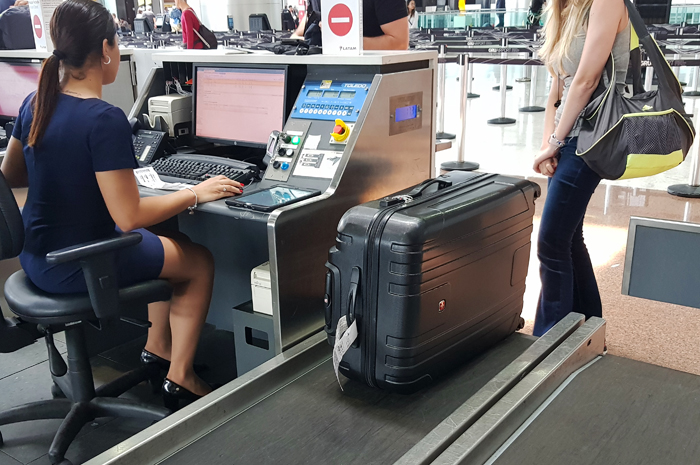
\includegraphics[width=0.4\textwidth]{imagens/viagem.png}
				
				\tiny{Fonte: Reprodução/Internet}
			\end{center}
			
			\centering
			\uncover<2->{
			\textit{Pois é: evitar isso é otimizar. É o que vamos aprender hoje com Algoritmos Genéticos.}
		}
			
		\end{frame}
	
		\begin{frame}{Introdução}
			\justifying
			\begin{block}{Conforme Alexandre Dias e André Gonçalves:}
				\begin{itemize}
					\item Passos inspirados no processo biológico de evolução;
					\uncover<2->{
					\item Ideia de sobrevivência dos mais adaptados - Charles Darwin (Origem das Espécies, 1859);
					} 
					\uncover<3->{
					\item Soluções cada vez melhores, a partir da evolução
					das gerações anteriores, até que uma solução
					próxima do ótimo seja obtida;
					}
					\uncover<4->{
					\item O método produz novas gerações melhores com
					base na medida de uma função de fitness;
					}
					\uncover<5->{
					\item Heurística inspirada na natureza;
					}
					
				\end{itemize}
			\end{block}
			
		\end{frame}
	
	
	\section{Estrutura de um AG}
	
		\begin{frame}{Estrutura de um AG}
			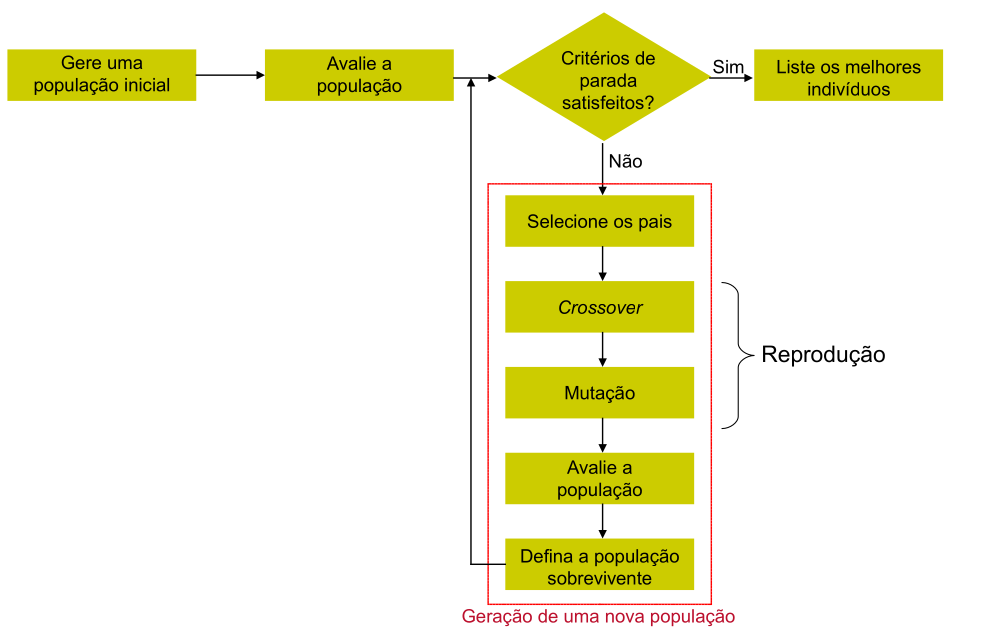
\includegraphics[scale=0.35]{imagens/estrutura.png}
		\end{frame}
	
	
		\begin{frame}{O Algoritmo Genético}
			\justifying
			Conforme Pozo et al. (2003), a ideia básica de funcionamento dos algoritmos genéticos é a de tratar as possíveis soluções do problema como indivíduos de uma população, que irá evoluir a cada iteração ou geração. Para isso é necessário construir um modelo de evolução onde os indivíduos sejam soluções de um problema.
		\end{frame}
	
	
		\begin{frame}{Algoritmo de um AG}
			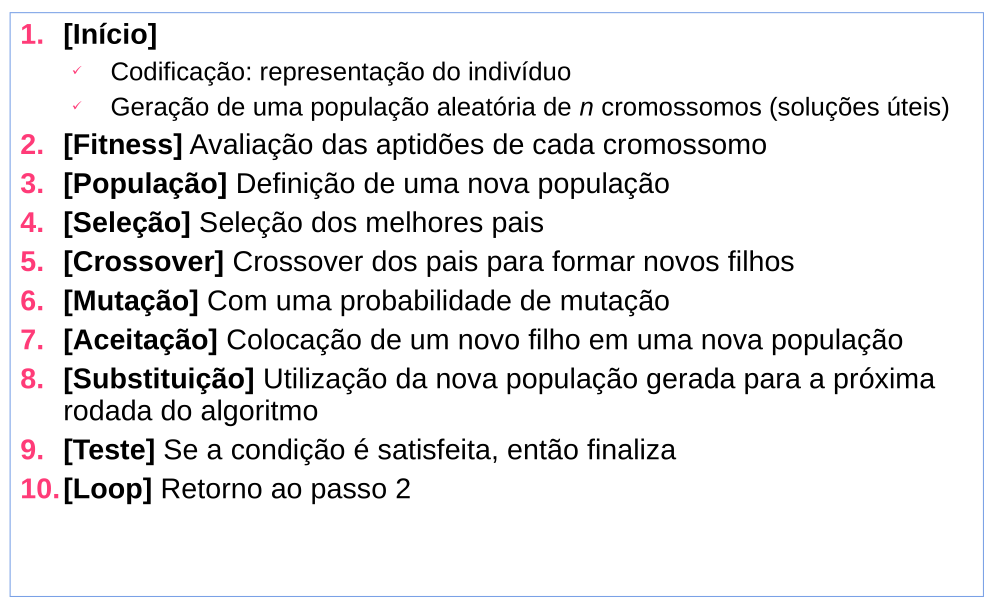
\includegraphics[scale=0.35]{imagens/algoritmo.png}
		\end{frame}
		
	
	\section{O problema da mochila (\textit{Knapsack Problem})}
	
		\begin{frame}{Problema da Mochila - (\textit{Knapsack Problem})}
			\begin{columns}
				\begin{column}{0.48\textwidth}
					\begin{itemize}
						\justifying
						\item Vários itens que gostaria de
						levar em uma mochila;
						\item Cada item com um peso e um
						benefício (valor);
						\item Há uma capacidade limite de
						peso;
						\item Deve-se carregar itens com o
						máximo valor total sem
						superar o limite de peso.
					\end{itemize}
				\end{column}
				
				\begin{column}{0.48\textwidth}
					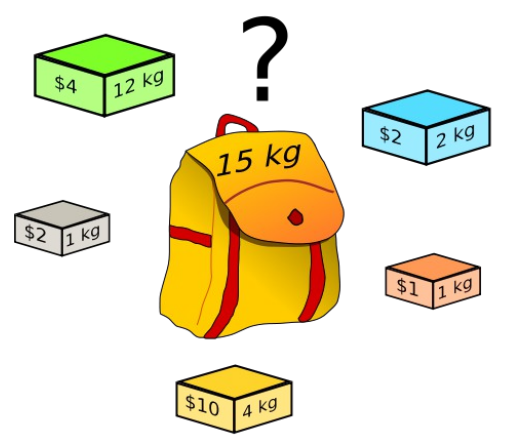
\includegraphics[scale=0.3]{imagens/mochila.png}
				\end{column}
			\end{columns}
		\end{frame}
		
		\begin{frame}{Problema da Mochila - (\textit{Knapsack Problem})}
			\justifying
			\begin{itemize}
				\item Problema de otimização combinatória (NP-Completo);
				\item Estudado por mais de um século (desde ~1897);
				\item Resolvido por variados algoritmos;
				\item Aplicações: gravação de arquivos desperdiçando o mínimo espaço em cada mídia, corte e empacotamento, por exemplo.
			\end{itemize}
		\end{frame}
		
		\begin{frame}{Problema da Mochila - (\textit{Knapsack Problem})}
			Exemplo:
			
			\begin{table}[h]
				\centering
				\begin{tabular}{l|c|c|c|c|c|c|c|}
					\hline
					Item & 1 & 2 & 3 & 4 & 5 & 6 & 7 \\
					\hline
					Benefício & 5 & 8 & 3 & 2 & 7 & 9 & 4 \\
					\hline
					Peso & 7 & 8 & 4 & 10 & 4 & 6 & 4 \\
					\hline
				\end{tabular}
				\caption{Itens do problema da mochila}
			\end{table}
			
			\begin{itemize}
				\item Mochila suporta, no máximo, (21+1) quilos;
				\item Adicione itens de modo a ter o máximo
				benefício.
			\end{itemize}
		\end{frame}
		
		
		
		\begin{frame}{Problema da Mochila - (\textit{Knapsack Problem})}
			\justifying
			\begin{itemize}
				\item Codificação: 0 = não existe; 1 = existe na mochila
				\item Cromossomo: 1010110 \\
			\end{itemize}
			\vspace{1mm}
			\centering
			\begin{tabular}{|c|c|c|c|c|c|c|c|}
				\hline
				\textbf{Item} & \textbf{1} & \textbf{2} & \textbf{3} & \textbf{4} & \textbf{5} & \textbf{6} & \textbf{7} \\
				\hline
				\textbf{Cromossomo} & 1 & 0 & 1 & 1 & 0 & 1 & 0 \\
				\hline
				\textbf{Existe?} & sim & não & sim & sim & não & sim & não \\
				\hline
			\end{tabular}
			 \vspace{2mm}
			
			\begin{itemize}
				\uncover<2->{
				\item Itens pego: 1,3,4 e 6.
				}
			\end{itemize}
			
		\end{frame}
		
		\begin{frame}{Problema da Mochila - (\textit{Knapsack Problem})}
			Geração aleatória de população com n cromossomos:
			
			\begin{enumerate}
				\item [a)] 0101010
				\item [b)] 1100100
				\item [c)] 0100011
			\end{enumerate}
		\end{frame}
		
		\begin{frame}{Problema da Mochila - (\textit{Knapsack Problem})}
			\justifying
			Aplicando função fitness \& seleção para o item a \\
			
			\centering
			\vspace{2mm}
			\begin{tabular}{|c|c|c|c|c|c|c|c|}
				\hline
				Item & 1 & 2 & 3 & 4 & 5 & 6 & 7 \\
				\hline
				Cromossomo & 0 & 1 & 0 & 1 & 0 & 1 & 0 \\
				\hline
				Benefício & 5 & 8 & 3 & 2 & 7 & 9 & 4 \\
				\hline
				Peso & 7 & 8 & 4 & 10 & 4 & 6 & 4 \\
				\hline
			\end{tabular}
			
			\vspace{2mm}
			\begin{itemize}
				\item [a)] Benefício = 19; Peso = 24 (\textit{Adeus, mochila! \textcolor{red}{\texttimes}})
			\end{itemize}
		\end{frame}
		
		\begin{frame}{Problema da Mochila - (\textit{Knapsack Problem})}
			\begin{block}{O que cabe na mochila?}
				\begin{enumerate}
					\item [b)] 1100100;
					
					\uncover<2->{
					\item [c)] 0100011;
					}
				\end{enumerate}
			\end{block}
			\vspace{2mm}
			
			\centering
			\begin{tabular}{|c|c|c|c|c|c|c|c|}
				\hline
				Item & 1 & 2 & 3 & 4 & 5 & 6 & 7 \\
				\hline
				Cromossomo &  &  &  &  &  &  &  \\
				\hline
				Benefício & 5 & 8 & 3 & 2 & 7 & 9 & 4 \\
				\hline
				Peso & 7 & 8 & 4 & 10 & 4 & 6 & 4 \\
				\hline
			\end{tabular}
			\vspace{2mm}
			
			\begin{itemize}
				\uncover<2->{
				\item [b)] Benefício = 20; Peso = 19 (\textit{solução viável $\checkmark$})
				}
			\end{itemize}
		\end{frame}
	
		\begin{frame}{Problema da Mochila - (\textit{Knapsack Problem})}
			\begin{block}{O que cabe na mochila?}
				\begin{enumerate}
					\item [c)] 0100011;
				\end{enumerate}
			\end{block}
			\vspace{2mm}
			
			\centering
			\begin{tabular}{|c|c|c|c|c|c|c|c|}
				\hline
				Item & 1 & 2 & 3 & 4 & 5 & 6 & 7 \\
				\hline
				Cromossomo &  &  &  &  &  &  &  \\
				\hline
				Benefício & 5 & 8 & 3 & 2 & 7 & 9 & 4 \\
				\hline
				Peso & 7 & 8 & 4 & 10 & 4 & 6 & 4 \\
				\hline
			\end{tabular}
			\vspace{2mm}
			
			\begin{itemize}
				\uncover<2->{
					\item [c)] Benefício = 21; Peso = 18 (\textit{solução ótima $\checkmark$})
				}
			\end{itemize}
			
			\centering
			\uncover<3->{Serão selecionados os cromossomos b e c.}
			
		\end{frame}		
		
		\begin{frame}{Problema da Mochila - (\textit{Knapsack Problem})}
			Compreendendo o processo de Crossover e mutação.
			
			$$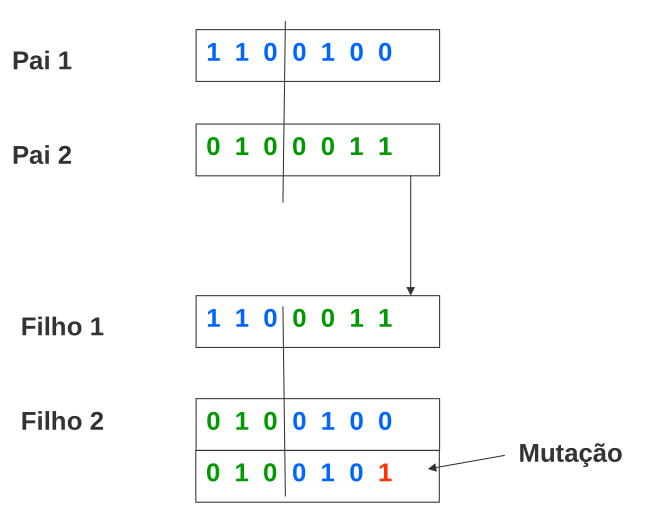
\includegraphics[scale=0.35]{imagens/crossover_mutacao.png}$$
		\end{frame}
	
	\section{AG na Prática com Excel}
	
		\begin{frame}{Considere a seguinte situação}
			\centering
			Seja $\mathbf{x} = (x_1, x_2, \ldots, x_7)$ um cromossomo, com $x_i \in \{0,1\}$.
			\textbf{Função objetivo (fitness):}
			\[
			f(\mathbf{x}) = \sum_{i=1}^{7} b_i x_i = 5x_1 + 8x_2 + 3x_3 + 2x_4 + 7x_5 + 9x_6 + 4x_7
			\]
			\textbf{Restrição:}
			\[
			g(\mathbf{x}) = \sum_{i=1}^{7} p_i x_i = 7x_1 + 8x_2 + 4x_3 + 10x_4 + 4x_5 + 6x_6 + 4x_7 \leq 22
			\]
			\begin{center}
				Maximizar $f(\mathbf{x})$ \quad sujeito a \quad $g(\mathbf{x}) \leq 22$
			\end{center}
		\end{frame}
\end{document}



